\documentclass[11pt]{article}
\usepackage{myz310e-notes}
\hypersetup{pdftitle={Linear classifiers and explicit feature maps},pdfauthor={Emre Onur Kahya},pdfsubject={MYZ 310E Machine Learning in Physics, Fall 2026, lecture note 9 (week 4)}}
\newcommand{\w}{\vect{w}}
\newcommand{\xt}{\tilde{\x}}

\begin{document}
\NoteTitle{9}{4}{Linear classifiers and\\ explicit feature maps}{Linear classifiers}{%
A linear classifier separates classes with a hyperplane. Many algorithms learn one --- nearest centroid, Gaussian
discriminant analysis, least squares, the perceptron, logistic regression, support vector machines --- and they differ
only in which hyperplane they choose. This note develops their geometry and their training, explains why a hyperplane
is often not enough, and shows the oldest way around it: map the inputs non-linearly and classify linearly in the new
space. Learning that map instead of fixing it is what a neural network does, the subject of week~5.}

\section{What makes a classifier linear}\label{sec:def}

A binary classifier is \emph{linear} if its decision function has the form
\[
  f(\x) = \operatorname{sign}\big(g(\x)\big), \qquad g(\x) = \w\T\x + b ,
\]
with labels $t \in \{-1, +1\}$, weight vector $\w \in \R^d$ and bias $b$. For $m$ classes, $f(\x) = \argmax_c
(W\x + \vect{b})_c$ with a weight matrix $W \in \R^{m \times d}$ and a bias vector; for $m = 2$ the two forms agree,
with $\w = W_{2:} - W_{1:}$ and $b = b_2 - b_1$ (Note~6, Section~1).

\paragraph{Geometry} The decision boundary $H = \{\x : \w\T\x + b = 0\}$ is a hyperplane --- a line in two dimensions, a
plane in three. The vector $\w$ is normal to it, and the signed distance of a point to $H$ is
\begin{equation}\label{eq:dist}
  r(\x) = \frac{\w\T\x + b}{\norm{\w}} ,
\end{equation}
so $g(\x)$ is a distance measured in units of $1/\norm{\w}$. The two decision regions are the half-spaces on either
side. In the multiclass case each region $\{\x : g_c(\x) > g_{c'}(\x)\ \forall c' \ne c\}$ is an intersection of
half-spaces, hence convex.

\paragraph{Linear separability} A dataset is \emph{linearly separable} if some hyperplane classifies all of it
correctly: there exist $\w, b$ with $t_i(\w\T\x_i + b) > 0$ for every $i$. Many datasets are not. The classic example is
XOR --- the points $(0,0)$ and $(1,1)$ in one class, $(0,1)$ and $(1,0)$ in the other --- which no line separates; its
discussion in Minsky and Papert's book of 1969 slowed research on neural networks for a decade~\cite{minsky1969}.

\section{Many roads to a hyperplane}\label{sec:roads}

The following algorithms all output a linear decision function; for the same data they choose different hyperplanes,
which generalise differently. Figure~\ref{fig:linclass} shows five of them on one dataset.

\paragraph{Nearest centroid} Store the class means $\vmu_c$ and assign $\x$ to the nearest. Since
$\norm{\x - \vmu_c}^2 = \norm{\x}^2 - 2\vmu_c\T\x + \norm{\vmu_c}^2$ and $\norm{\x}^2$ is common to all classes, the
rule is linear with $\w_c = 2\vmu_c$ and $b_c = -\norm{\vmu_c}^2$; for two classes the boundary is the perpendicular
bisector of the segment between the means.

\paragraph{Gaussian discriminant analysis} With Gaussian classes sharing one covariance, the Bayes classifier is
linear, $\w = \Sigma^{-1}(\vmu_1 - \vmu_0)$ (Note~6, Section~3). It accounts for the shape of the classes, which
nearest centroid ignores. Fisher's linear discriminant, derived differently --- the projection that best separates the
class means relative to the spread within classes --- gives the same direction.

\paragraph{Least squares on $\pm 1$ targets} Nothing prevents fitting linear regression (Note~8) to the labels $t_i$ and
classifying by the sign of the prediction. But squared error penalises points that are correctly classified \emph{with
a large margin}, since their prediction is far from $\pm 1$. A distant cluster of easy examples therefore pulls the
boundary towards itself; in Figure~\ref{fig:linclass} the twelve far-away amber points tilt the least-squares line and
triple its training error (9.8\%) compared with logistic regression (3.3\%).

\begin{figure}[h]
\centering
\begin{minipage}[c]{0.6\linewidth}
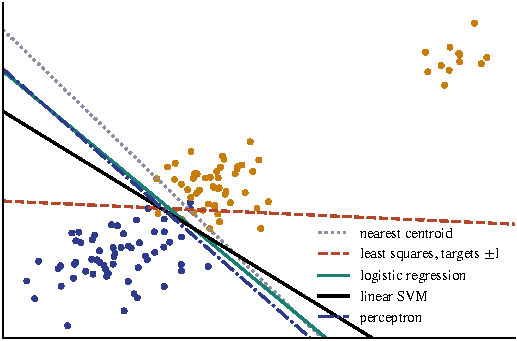
\includegraphics[width=\linewidth]{figures/linear_classifiers.pdf}
\end{minipage}\hfill
\begin{minipage}[c]{0.37\linewidth}
\caption{Five linear classifiers on the same 122 points. All boundaries are straight lines, but they differ.
Training errors: nearest centroid 4.9\%, least squares 9.8\%, logistic regression, linear SVM and perceptron 3.3\%.
The least-squares line is pulled by the distant amber cluster in the top right.}
\label{fig:linclass}
\end{minipage}
\end{figure}

\paragraph{Minimising the error directly} The training error rate is piecewise constant in $(\w, b)$: its
gradient is zero almost everywhere and gradient descent (Note~7) cannot move. The remaining algorithms minimise
surrogates (Note~4, Section~2) that do have useful gradients.

\section{The perceptron}\label{sec:perceptron}

Rosenblatt's perceptron~\cite{rosenblatt1958}, built in hardware as the Mark~I in the late 1950s, was one of the first
learning machines and the first artificial neuron trained from data. Starting from $\w = \vect{0}$, $b = 0$, it visits
the examples in random order and corrects mistakes:
\begin{algorithmic}[1]
\Repeat
  \For{each $(\x_i, t_i)$ in random order}
    \If{$t_i(\w\T\x_i + b) \le 0$} $\w \gets \w + t_i\x_i$, \quad $b \gets b + t_i$ \EndIf
  \EndFor
\Until{no mistakes in a full pass (or a maximum number of passes)}
\end{algorithmic}
This is stochastic gradient descent with step $\eta = 1$ on the \emph{perceptron criterion}
\[
  J(\w, b) = \sum_{i\ \text{misclassified}} -t_i(\w\T\x_i + b),
\]
which measures how far misclassified points lie on the wrong side. If the data are separable with margin $\gamma$ (some unit-norm $\w^*$ has $t_i \w^{*\mathsf{T}}\x_i \ge \gamma$)
and $\norm{\x_i} \le R$, the perceptron makes at most $(R/\gamma)^2$ mistakes before separating them~\cite{novikoff1962}
--- a bound independent of $n$ and $d$. If the data are not separable it never stops: on the data of
Figure~\ref{fig:linclass} it made 606 corrections in 100 passes. It also stops at \emph{any} separating hyperplane,
however close to the data, which motivates the margin of Section~\ref{sec:svm}.

\section{Logistic regression}\label{sec:logistic}

Despite its name, logistic regression~\cite{cox1958} is a classifier. With $t \in \{0, 1\}$ it models the class
probability directly,
\[
  P(t = 1 \mid \x) = \sigma(\w\T\x + b), \qquad \sigma(z) = \frac{1}{1 + e^{-z}} ,
\]
the logistic sigmoid, a smooth version of a step function that maps the score to $(0, 1)$. It is trained by minimising
the cross-entropy (Note~4, Section~2), the negative log-likelihood of the labels. With $y_i = \sigma(\w\T\xt_i)$ and the
bias absorbed as in Note~8,
\[
  J(\w) = -\sum_{i=1}^n \big[t_i \log y_i + (1 - t_i)\log(1 - y_i)\big], \qquad
  \nabla J = \sum_{i=1}^n (y_i - t_i)\, \xt_i .
\]
The gradient has the same form as for least squares --- prediction minus target, times input --- because $\sigma' =
\sigma(1 - \sigma)$ cancels a factor. The objective is convex, but $\nabla J = \vect{0}$ has no closed-form solution; it is
minimised by gradient descent, by mini-batch SGD for large data, or by Newton's method (Note~7), which converges in a few
iterations. Two practical points: if the data are separable, $\norm{\w}$ grows without bound because sharper sigmoids keep
lowering the loss, so a ridge penalty (Note~8) is added; and with $m$ classes the sigmoid becomes the \emph{softmax},
$P(t = c \mid \x) = e^{g_c(\x)}/\sum_{c'} e^{g_{c'}(\x)}$, trained with the categorical cross-entropy.

Since $\sigma(z) > \frac12$ exactly when $z > 0$, predicting the most probable class is still $\operatorname{sign}(\w\T\x +
b)$: the boundary is a hyperplane. What logistic regression adds is a calibrated probability, and a loss that, unlike
squared error, does not punish confident correct predictions. In neural terms it is a single neuron with a sigmoid
activation.

\begin{modern}{every neural classifier ends in logistic regression}
The last layer of an image classifier or a language model is a linear map followed by a softmax: multiclass logistic
regression on features computed by the layers below. Conversely, training only a logistic regression on the frozen
features of a pre-trained network --- a \emph{linear probe} --- is the standard way to measure what those features
contain~\cite{alain2017}; CLIP, for instance, was evaluated with linear probes on 27 datasets~\cite{radford2021}. Everything
in this note therefore applies on top of the most modern representations.
\end{modern}

\section{Support vector machines}\label{sec:svm}

Among all separating hyperplanes, the \emph{maximum-margin} one stays as far as possible from the closest training
points. The \emph{functional margin} of an example is $t_i g(\x_i)$ --- positive if it is correctly classified, large if
confidently so --- and its \emph{geometric margin} is $t_i g(\x_i)/\norm{\w}$, its signed distance to the boundary by
\eqref{eq:dist}. Since rescaling $(\w, b)$ does not move the hyperplane, we may fix the smallest functional margin to one;
maximising the geometric margin $1/\norm{\w}$ then becomes the \emph{hard-margin SVM}:
\[
  \min_{\w, b} \tfrac12 \norm{\w}^2 \quad \text{subject to} \quad t_i(\w\T\x_i + b) \ge 1, \quad i = 1, \dots, n,
\]
a quadratic programme with linear constraints~\cite{cortes1995}. For data that are not separable, \emph{slack} variables
$\xi_i \ge 0$ allow violations at a price: minimise $\frac12\norm{\w}^2 + C\sum_i \xi_i$ subject to $t_i(\w\T\x_i + b)
\ge 1 - \xi_i$. Eliminating the slacks gives an unconstrained form,
\[
  \min_{\w, b} \; \sum_{i=1}^n \max\big(0,\, 1 - t_i(\w\T\x_i + b)\big) + \frac{1}{2C}\norm{\w}^2 ,
\]
the hinge loss of Note~4 plus a ridge penalty. The hyperparameter $C$ trades margin against training errors; $C \to \infty$
recovers the hard margin.

\begin{figure}[h]
\centering
\begin{minipage}[c]{0.4\linewidth}
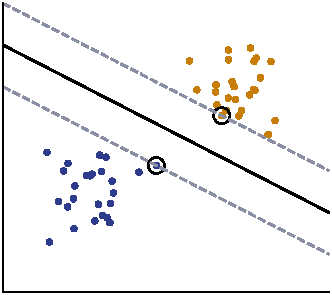
\includegraphics[width=\linewidth]{figures/margin.pdf}
\end{minipage}\hfill
\begin{minipage}[c]{0.56\linewidth}
\caption{A maximum-margin classifier. The dashed lines are $g(\x) = \pm 1$; the margin between them has width
$2/\norm{\w}$. Only the two circled points --- the support vectors --- determine the solution: moving any other point,
without crossing the dashed lines, changes nothing.}
\label{fig:margin}
\end{minipage}
\end{figure}

\paragraph{Support vectors} The solution has the form $\w = \sum_i \alpha_i t_i \x_i$ with $\alpha_i \ge 0$, and only
points on or inside the margin have $\alpha_i > 0$ (Figure~\ref{fig:margin}). These \emph{support vectors} are usually a
small fraction of the data. Because $\w$ is a combination of training inputs, the problem can be rewritten in terms of the
$\alpha_i$ and inner products $\x_i\T\x_j$ alone --- the dual formulation, which opens the way to the kernel trick of
Section~\ref{sec:features}. Soft-margin SVMs, linear or kernelised, were among the most widely used classifiers of the
2000s: good accuracy, a convex problem and few hyperparameters.

\paragraph{More than two classes} Binary classifiers extend in two standard ways: \emph{one-against-all}, with $m$
classifiers each separating one class from the rest and the highest score winning; and \emph{one-against-one}, with
$m(m-1)/2$ pairwise classifiers and a vote. Taking the highest score, rather than the raw yes/no answers, avoids the
ambiguous regions where several or no classifiers claim a point.

\section{Beyond linear: explicit feature maps}\label{sec:features}

Whatever the algorithm, a linear classifier draws a hyperplane, and its capacity is limited. The oldest remedy keeps
the linear algorithm and changes the space: apply a fixed non-linear \emph{feature map} $\phi : \R^d \to \R^D$ and learn a
linear classifier on $\phi(\x)$,
\[
  f(\x) = \operatorname{sign}\big(\w\T\phi(\x) + b\big) .
\]
The boundary is a hyperplane in the new space and a curved surface in the original one. For two inputs, the quadratic
map $\phi(x_1, x_2) = (x_1^2, x_2^2, x_1x_2, x_1, x_2)$ makes $\w\T\phi(\x) + b$ an arbitrary second-degree polynomial,
so the boundary can be any conic. In Figure~\ref{fig:fmap} a class that surrounds the other defeats logistic regression
on $\x$ (49\% training error, chance level), while the same algorithm on $\phi(\x)$ separates the classes perfectly
with a circle.

\begin{figure}[h]
\centering
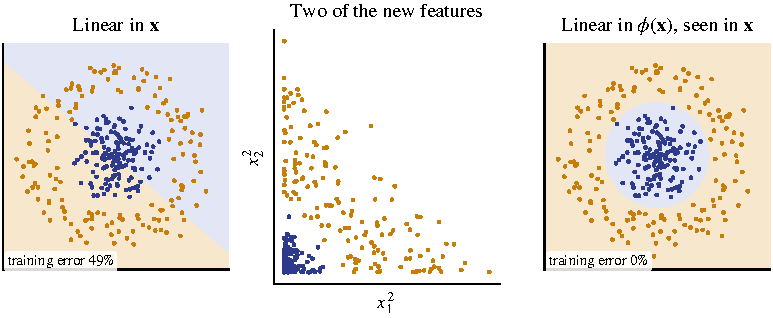
\includegraphics[width=\linewidth]{figures/feature_map.pdf}
\caption{Left: logistic regression on the raw inputs. Centre: two of the five quadratic features, in which the classes
are separated by a straight line. Right: logistic regression on all five quadratic features, with the boundary drawn in
the original coordinates.}
\label{fig:fmap}
\end{figure}

\paragraph{The cost of explicit maps} All monomials of degree at most $p$ in $d$ variables number $\binom{d+p}{p}$:
21 for $d = 2, p = 2$, but $176\,851$ for $d = 100, p = 3$. The capacity grows accordingly, and with it the need for
regularisation and data (Note~4) --- the curse of dimensionality in a new form (Note~3). There are three ways to obtain a
non-linear feature map:
\begin{enumerate}
\item \textbf{Choose it explicitly}, a priori, as above: polynomials, physically motivated variables, or random
non-linear features --- the random ReLU features of Note~4, Section~8, are an example, and random Fourier features
approximate kernel machines at large scale~\cite{rahimi2007}.
\item \textbf{Choose it implicitly} through a kernel $k(\x, \x') = \phi(\x)\T\phi(\x')$: algorithms that need only inner
products, like the dual SVM, can work in very high or even infinite-dimensional feature spaces without ever computing
$\phi$ (kernel SVM, kernel logistic regression).
\item \textbf{Learn it}: let $\phi$ have its own parameters and fit them together with $\w$. A multilayer perceptron
does exactly this, $f(\x) = \w\T a(V\x + \vect{c}) + b$, with a learned matrix $V$ and an element-wise non-linearity
$a$: a linear classifier on features that are themselves trained by gradient descent (Note~7). This is where week~5
begins.
\end{enumerate}

\begin{physics}{feature engineering, the physicist's way}
The invariant mass of a pair of photons, $m_{\gamma\gamma}^2 = 2E_1E_2(1 - \cos\theta_{12})$, is a non-linear feature map of
the measured energies and angles. In it, a Higgs boson decaying to two photons is a narrow peak, and a simple window
separates much of the signal --- something no hyperplane in the raw measurements could do. Physics has always supplied such
features. When deep networks were given only low-level detector quantities in benchmark searches for new particles, they
matched or exceeded the performance obtained with the best hand-engineered variables, having learned equivalent features
themselves~\cite{baldi2014}.
\end{physics}

\begin{keyidea}[Summary]
A linear classifier predicts $\operatorname{sign}(\w\T\x + b)$; its boundary is a hyperplane normal to $\w$, and
$g(\x)/\norm{\w}$ is a signed distance. Nearest centroid, LDA, least squares, the perceptron, logistic regression and
the SVM all learn hyperplanes, chosen by different criteria: least squares is pulled by distant points, the perceptron
stops at any separator, logistic regression gives calibrated probabilities with a convex loss, and the SVM maximises the
margin and depends only on its support vectors. A non-linear feature map makes linear methods non-linear: chosen
explicitly, implicitly through kernels, or learned, as in a neural network.
\end{keyidea}

\begin{exercises}
\item Show that $\w$ is normal to the hyperplane $\w\T\x + b = 0$ and derive the distance formula \eqref{eq:dist}. What is
the distance from the origin to the hyperplane?
\item Show that the XOR points are not linearly separable, and find a single extra feature $\phi_3(\x)$ such that they
become separable in $(x_1, x_2, \phi_3)$.
\item Derive $\nabla J$ for logistic regression using $\sigma' = \sigma(1 - \sigma)$, and the Hessian
$\sum_i y_i(1 - y_i)\,\xt_i\xt_i\T$. Conclude that $J$ is convex. Why does $\norm{\w}$ diverge on separable data?
\item Implement the perceptron and run it on separable data with margin $\gamma$ and radius $R$ of your choice. Compare
the number of mistakes with the bound $(R/\gamma)^2$.
\item Explain why the solution of the soft-margin SVM does not change when a correctly classified point outside the
margin is moved, as long as it stays outside the margin. Which points of Figure~\ref{fig:linclass} would a linear SVM
ignore?
\item How many features does the full polynomial map of degree~3 produce for $28 \times 28$ images? Estimate the memory
needed to store them for $60\,000$ images in 32-bit floats, and suggest an alternative.
\end{exercises}

\paragraph{Further reading} Bishop~\cite{bishop2006}, chapter~4 and section~7.1; Hastie, Tibshirani and
Friedman~\cite{hastie2009}, sections~4.4--4.5 and~12.2--12.3; for the history of the perceptron, Rosenblatt~\cite{rosenblatt1958}.

\begin{thebibliography}{99}\small
\bibitem{alain2017} G.~Alain and Y.~Bengio, Understanding intermediate layers using linear classifier probes, \emph{ICLR Workshop} (2017).
\bibitem{baldi2014} P.~Baldi, P.~Sadowski and D.~Whiteson, Searching for exotic particles in high-energy physics with deep learning, \emph{Nat.\ Commun.}\ 5, 4308 (2014).
\bibitem{bishop2006} C.~M. Bishop, \emph{Pattern Recognition and Machine Learning}, Springer (2006).
\bibitem{cortes1995} C.~Cortes and V.~Vapnik, Support-vector networks, \emph{Mach.\ Learn.}\ 20, 273--297 (1995).
\bibitem{cox1958} D.~R. Cox, The regression analysis of binary sequences, \emph{J.\ R.\ Stat.\ Soc.\ B} 20, 215--242 (1958).
\bibitem{hastie2009} T.~Hastie, R.~Tibshirani and J.~Friedman, \emph{The Elements of Statistical Learning}, 2nd ed., Springer (2009).
\bibitem{minsky1969} M.~Minsky and S.~Papert, \emph{Perceptrons}, MIT Press (1969).
\bibitem{novikoff1962} A.~B.~J. Novikoff, On convergence proofs on perceptrons, \emph{Proc.\ Symposium on the Mathematical Theory of Automata} 12, 615--622 (1962).
\bibitem{radford2021} A.~Radford \emph{et al.}, Learning transferable visual models from natural language supervision, \emph{ICML} (2021).
\bibitem{rahimi2007} A.~Rahimi and B.~Recht, Random features for large-scale kernel machines, \emph{NeurIPS} (2007).
\bibitem{rosenblatt1958} F.~Rosenblatt, The perceptron: a probabilistic model for information storage and organization in the brain, \emph{Psychol.\ Rev.}\ 65, 386--408 (1958).
\end{thebibliography}

\SourceNote
\end{document}
